\documentclass[pdf, aspectratio=169]{beamer}
\usepackage[]{hyperref,graphicx,siunitx,lmodern,booktabs,tikz,wasysym}
\usepackage{pdfpc-commands}

\usepackage[mode=buildnew]{standalone}
\mode<presentation>{\usetheme{Astro}}

\graphicspath{ {../Images/} }

\sisetup{per-mode=symbol}
\usetikzlibrary{calc, shapes.geometric}

\newcommand<>{\boxalert}[1]{\alt#2{\colorbox{Blue}{\color{LOrange}#1}}{#1}}

%preamble
\title{Where in the World?}
\date{September 5, 2018}
\author{Jed Rembold}

\begin{document}
\renewcommand*{\theenumi}{\Alph{enumi}}

\begin{frame}{Announcements}
	\begin{itemize}
	  \item New homework on WebWorK posted after class, due Friday
		  \begin{itemize}
		  	\item The required Nautical Almanac will be posted on our website
		  \end{itemize}
	  \item Most of you look like you are keeping up with the WebWorK, so keep it up! For those of you a little behind, ask questions, set aside time, but I highly recommend getting caught up sooner rather than later!
	  \item Polling: \url{rembold-class.ddns.net}
	\end{itemize}
\end{frame}

\begin{frame}{Tonight's Sky}
  \begin{itemize}
	  \item ISS crossing tomorrow morning
		  \begin{itemize}
			  \item About 5:02 am, about \ang{34} above the horizon to the North
		  \end{itemize}
	  \item Iridium flare tonight at 10:27pm
		  \begin{itemize}
		  	\item Almost dead zenith
			\item Near the bright star Vega which is basically looking straight up
			\item Much brighter ones coming later in the week
		  \end{itemize}
  \end{itemize}
  \begin{center}
	\inlineMovie{../Videos/IridiumFlare.ogv}{../Videos/IridiumFlare.png}{width=.52\textwidth}
  \end{center}
\end{frame}

\begin{frame}{Review Question}
	What was one of the main reasons for Ptolomy improving Aristotle's geocentric model of the Solar System with his own circles-in-circles model?
  \begin{enumerate}
	\item The Sun moved opposite through the sky from the planets
	\item \alert<2>{Some planets occasionally moved backwards through the sky for part of the year}
	\item The orbit of Neptune was observed to be non-circular
	\item The Sun was determined to be in the center of the Solar System.
  \end{enumerate}
\end{frame}

\begin{frame}{A Detour}
  We'll return to the Greeks soon, but now for a small aside:
  \begin{itemize}
	\item Finding the circumference of the Earth via Astronomy is great
	\item Finding your location on the globe via Astronomy is even greater!
	  \begin{itemize}
		\item These techniques are technically a jump forward in the timeline
		\item Largely in the spirit of ``what can primitive astronomy tell me?''
	  \end{itemize}
  \end{itemize}
  \begin{center}
	\begin{tikzpicture}
	  \node at (0,0) {\includegraphics[width=4cm]{world.png}};
	  \foreach \x in {1,2,...,5}{
		\node[black, rotate=rand*30] at (rand*360:rand*2) {?};
	  }
	\end{tikzpicture}
  \end{center}
\end{frame}

\begin{frame}{The Easy Step: Latitude}
  \begin{itemize}
	\item Location in the sky of celestial poles varies with latitude
	\item Altitude of celestial pole in the local sky gives your latitude
	  \begin{itemize}
		\item Northern Hemisphere - North Star / Polaris
		\item Southern Hemisphere - 4 Lengths from the Southern Cross / Crux
	  \end{itemize}
  \end{itemize}
  \begin{center}
	\includegraphics[width=.4\textwidth]{ch3_star_trail.jpeg}
	\includegraphics[width=.4\textwidth]{ch3_star_trail_S.jpg}
  \end{center}
\end{frame}

\begin{frame}{The Harder Step: Longitude}
  \begin{itemize}
	\item Our latitude is ``fixed'' with respect to the stars, so the celestial pole is always as the same angle
	\item Our longitude is not fixed, because the Earth is rotating
	  \begin{itemize}
		\item You can also think of longitude being determined by where the Prime Meridian is, and that is always rotating
	  \end{itemize}
	\item Requires us to use some different machinery to determine longitude
	\item We need to add \alert{time} to our machinery in addition to a view of the sky
  \end{itemize}
\end{frame}

\begin{frame}{Determining Longitude}
  Bert and Ernie are hanging out at the same latitude, but different longitudes. At midnight, Bert sees the star Vega directly overhead. Five hours later, Ernie sees the star Vega directly overhead.
  \begin{center}
	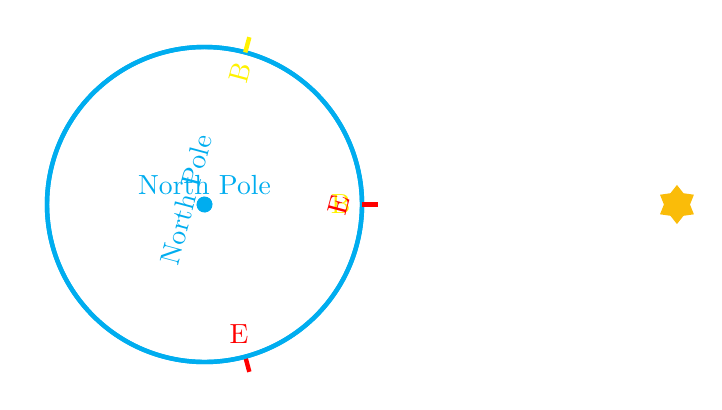
\begin{tikzpicture}
	  \node[fill=yellow!50!orange, star, star points=6] at (6,0) {};
	  \draw[white, dashed] (2.5,0) -- (5.5,0);
	  \onslide<1>{
		\begin{scope}
		  \fill[cyan] (0,0) circle (1mm) node[above] {North Pole};
		  \draw[cyan, ultra thick] (0,0) circle (2cm);
		  \draw[yellow, ultra thick] (0:2) node[left] {B} -- +(0:2mm);
		  \draw[red, ultra thick] (-75:2) node[shift=(105:3mm)] {E} -- +(-75:2mm);
		\end{scope}
		\node[white!90] at (5,-1.5) {\LARGE1:00am};
	  }
	  \onslide<2>{
		\begin{scope}[rotate=75, transform shape]
		  \fill[cyan] (0,0) circle (1mm) node[above] {North Pole};
		  \draw[cyan, ultra thick] (0,0) circle (2cm);
		  \draw[yellow, ultra thick] (0:2) node[left] {B} -- +(0:2mm);
		  \draw[red, ultra thick] (-75:2) node[shift=(105:3mm)] {E} -- +(-75:2mm);
		\end{scope}
		\node[white!90] at (5,-1.5) {\LARGE6:00am};
	  }
	\end{tikzpicture}
  \end{center}
\end{frame}

\begin{frame}{Determining Longitude: Part 2}
  \begin{itemize}
	\item This 5 hour difference ``fixes'' their longitude positions on Earth relative to one another
	\item Recall 1 hour $\approx$ \SI{15}{\degree}
	\item If Bert was at the Prime Meridian, Ernie would be \SI{75}{\degree} West
  \end{itemize}
  \pause
  \begin{alertblock}{Problem!}
	But what about when we don't have a friend conveniently located on the Prime Meridian?
  \end{alertblock}
\end{frame}

\begin{frame}{Your New Friend: The Nautical Almanac}
  \begin{itemize}
	\item Is very old: since 1767
	\item Keeps tabs of where important things in the sky should be, every hour, every day
	\item Values are as \alert{if the observer was at the prime meridian}
	\item Many complicated ways to use the almanac
	  \begin{itemize}
		\item Are you moving?
		\item Where do you see your reference star?
		\item Can you accurately see the horizon?
	  \end{itemize}
	\item We'll take the simplest course of action
	  \begin{itemize}
		\item Not moving, horizon visible, reference star crossing meridian
	  \end{itemize}
  \end{itemize}
\end{frame}

\begin{frame}{Some Vocabulary}
  \begin{itemize}
	\item The \alert{Hour Angle}: the number of degrees West of the meridian an object appears
	\item \alert{GHA} = Greenwich Hour Angle: Where the object appears as seen on the Prime Meridian
	\item \alert{LHA} = Local Hour Angle: Where the object appears as seen where you are standing
	  \begin{itemize}
		\item We will be using stars crossing our meridian, so the LHA will always be zero for us!
	  \end{itemize}
	\item In general:
	  \[\text{LHA } = \text{ GHA } - \text{ Longitude W of Prime Meridian }\]
  \end{itemize}
\end{frame}

\begin{frame}{One Last Wrinkle}
  \begin{itemize}
	\item Listing the GHA of every reference star at every hour of every day would require a huge book
	\item The stars do not move relative to one another, so most of that information would be redundant
	\item Almanac gives us a star's \alert{SHA} (Sidereal Hour Angle)
	\item This is an angle given relative to the constellation Aries
	\item Almanac just gives the GHA for Aries, and lets you work it out for the other reference stars
	  \[\text{GHA Star} = \text{SHA Star} + \text{GHA Aries}\]
  \end{itemize}
\end{frame}

\begin{frame}{A Note on Time}
  \begin{itemize}
	\item Recall that you'll need to use the time to look up the GHA of Aries in the Almanac
	\item All of these times \alert{need to be in UTC} (aka Greenwich time GMT)
	\item This is so we can have a single, synchronized clock
	\item This method does assume that you have some method of knowing this time
	  \begin{itemize}
		\item This seems reasonable if you go somewhere planning to need to navigate yourself
		\item Maybe less reasonable if you suddenly find yourself in a foreign place
	  \end{itemize}
	\item Morale of the Story: Get the almanac tattooed and a tiny watch embedded in your skin\ldots
  \end{itemize}
\end{frame}

\begin{frame}{Jed's 8 Step Plan to Find Yourself}
  \begin{enumerate}
	\item Are you in the Northern or Southern Hemisphere? (Do you see the North Star or Southern Cross?)
	\item Measure angle to celestial pole to get latitude (negative if Southern Hemisphere)
	\item In \alert{opposite} direction, find a reference star very near the meridian (North-South line)
	\item What is the time and date? Find the appropriate page and line in the almanac.
	\item Calculate your reference star's GHA
	\item Calculate your raw longitude in degrees West of the Prime Meridian
	\item If larger than 360, subtract 360.
	\item If still larger than 180, you are East of the Prime Meridian instead of West. Subtract 360 \alert{again} to get your Longitude West of Prime Meridian (it will be negative!)
  \end{enumerate}
\end{frame}

\begin{frame}{Example!}
  \begin{example}
	Salem is at \SI{44.9}{\degree N} and \SI{123.0}{\degree W}. At 5:00am on 9/6/2017 UTC, we took two images of the night sky.
  \end{example}
\end{frame}

\begin{frame}{The Images}
  \begin{center}
	\includegraphics[width=.38\textwidth]{ch3_SalemN.pdf}
	\includegraphics[width=.38\textwidth]{ch3_SalemS.pdf}
  \end{center}
\end{frame}

\begin{frame}{The Process}
  \begin{enumerate}
	\item Are you in the Northern or Southern Hemisphere? (Do you see the North Star or Southern Cross?)
	  \begin{itemize}
		\item<2-> I see the North Star, so Northern Hemisphere
	  \end{itemize}
	\item Measure angle to celestial pole to get latitude (negative if Southern Hemisphere)
	  \begin{itemize}
		\item <3-> The North Star is barely under \SI{45}{\degree}. We'll call it \SI{+44.5}{\degree N}
	  \end{itemize}
	\item In \alert{opposite} direction, find a reference star very near the meridian (North-South line)
	  \begin{itemize}
		\item <4-> Looks like Altair is lying right on the Meridian and is one of our reference options!
	  \end{itemize}
	\item What is the time and date? Find the appropriate page and line in the almanac.
	  \begin{itemize}
		\item <5-> It is September 6, 2016 at 5:00 UTC. This is on page 168 of the almanac.
	  \end{itemize}
  \end{enumerate}
\end{frame}

\begin{frame}{Step E}
  \vspace{-1cm}
  \begin{columns}
	\column{.4\textwidth}
	\begin{itemize}
	  \item<1-> Find Altair
	  \item<2-> Note SHA
	  \item<3-> Find time line
	  \item<4-> Read GHA of Aries
	\end{itemize}
	\column{.5\textwidth}
	\begin{center}
	  \begin{tikzpicture}
		\node at (0,0) {\includegraphics[width=.8\textwidth]{ch3_SalemAlmanac.pdf}};
		%\draw[red] (-2,-2) grid (2,2);
		\draw<1>[thick, cyan,fill=cyan!50, fill opacity=0.2] (12mm,-9.3mm) rectangle +(4mm,.8mm);
		\draw<2>[thick, cyan,fill=cyan!50, fill opacity=0.2] (16mm,-9.3mm) rectangle +(3.5mm,.8mm);
		\draw<3>[thick, cyan,fill=cyan!50, fill opacity=0.2] (-25.6mm,-15.97mm) rectangle +(2mm,.8mm);
		\draw<4>[thick, cyan,fill=cyan!50, fill opacity=0.2] (-23.2mm,-15.97mm) rectangle +(3.5mm,.8mm);
	  \end{tikzpicture}
	\end{center}
  \end{columns}
  
\end{frame}

\begin{frame}{Process Cont'd}
  \begin{enumerate}
	\setcounter{enumi}{4}
	\item Calculate your reference star's GHA
	  \begin{itemize}
		\item <2-> Altair has a SHA of \SI{62}{\degree} \SI{5.3}{\arcminute} = \SI{62.0883}{\degree}. At this time, the GHA of Aries is \SI{60}{\degree} \SI{28.9}{\arcminute} = \SI{60.4817}{\degree}. Thus
		  \[\text{GHA Altair} = \SI{62.0883}{\degree} + \SI{60.4817}{\degree} = \SI{122.57}{\degree}\]
	  \end{itemize}\vspace{-5mm}
	\item Calculate your raw longitude in degrees West of the Prime Meridian
	  \begin{itemize}
		\item <3-> Since our LHA is 0, our measured GHA of Altair equals our longitude W!
	  \end{itemize}
	\item If larger than 360, subtract 360.
	  \begin{itemize}
		\item <4-> No need for anything else!
	  \end{itemize}
  \end{enumerate}
  \begin{block}{The Final Tally}<5->
	We determined that Salem is at \SI{44.5}{\degree N} and \SI{122.6}{\degree W}. Not too shabby!
  \end{block}
\end{frame}

\begin{frame}{I'd like another!}
  \begin{example}
	Buenos Aires is located at \SI{34.57}{\degree S} and \SI{58.36}{\degree W}. You take two images at 23:00 on October 14, 2017 UTC. Find the latitude and longitude of Buenos Aires as determined by your stars and almanac, and compare to the actual value.
  \end{example}
\end{frame}

\begin{frame}{Buenos Aires Promptings}
  \begin{itemize}[<+->]
	\item The Southern Cross is visible
	\item A line from the Southern cross to the meridian intersects at about \SI{32}{\degree}
	\item The reference star Deneb is visible to the North
	\item At the time given, the GHA of Aries is \SI{8}{\degree} \SI{40.5}{\arcminute}
	\item The corresponding GHA of Deneb at this time is \SI{58.16}{\degree}
  \end{itemize}
\end{frame}

\end{document}
